\section{Bestimmung des Verstärkungsfaktor des laseraktiven Mediums}
\subsection{Messung der Intensität}
In diesem Versuchsteil soll der Verstärkungsfaktor $\nu$ des Lasers bestimmt werden.
Dazu wird ein kippbares Glasplättchen in den Resonator eingebracht.
Das Plättchen erzeugt zusätzliche Verluste, durch winkelabhängige Reflexion.
Der Laser wird hierbei mit einer möglichst großen Leistung (in unserem Fall $\left(4,32\pm0,02\right)\,\text{mW}$) betrieben.\\

Zunächst haben wir die Nullstellung des Drehtisches bestimmt.
Bei dieser steht das Glasplättchen vertikal und der Laserstahlt wird somit in sich zurück reflektiert.\\
In unserem Fall folgt für $\alpha_0$:
\begin{equation}
    \alpha_0=21,12\,^\circ
\end{equation}
Durch Drehung des Glasplättchens wird die Laserstrahlung $I_L(\alpha)$ und die am Plättchen reflektierte Intensität $I_R(\alpha)$ moduliert.
Zur Messung der Intensität wird der Laserstahl noch mittels eines Umlenkspiegels auf die Photodiode justiert.
Das Messprogramm verfährt nun den Spiegel und misst in Abhängigkeit des Winkels die transmittierte Intensität.
Von den gemessenen Winkeln wird der Kalibrierungswinkel $\alpha_0$ abgezogen.\\
Somit ergibt sich folgender Verlauf:
\begin{figure}[h]
  \centering\scalebox{1.1}{% GNUPLOT: LaTeX picture with Postscript
\begingroup
  % Encoding inside the plot.  In the header of your document, this encoding
  % should to defined, e.g., by using
  % \usepackage[cp1252,<other encodings>]{inputenc}
  \inputencoding{cp1252}%
  \makeatletter
  \providecommand\color[2][]{%
    \GenericError{(gnuplot) \space\space\space\@spaces}{%
      Package color not loaded in conjunction with
      terminal option `colourtext'%
    }{See the gnuplot documentation for explanation.%
    }{Either use 'blacktext' in gnuplot or load the package
      color.sty in LaTeX.}%
    \renewcommand\color[2][]{}%
  }%
  \providecommand\includegraphics[2][]{%
    \GenericError{(gnuplot) \space\space\space\@spaces}{%
      Package graphicx or graphics not loaded%
    }{See the gnuplot documentation for explanation.%
    }{The gnuplot epslatex terminal needs graphicx.sty or graphics.sty.}%
    \renewcommand\includegraphics[2][]{}%
  }%
  \providecommand\rotatebox[2]{#2}%
  \@ifundefined{ifGPcolor}{%
    \newif\ifGPcolor
    \GPcolorfalse
  }{}%
  \@ifundefined{ifGPblacktext}{%
    \newif\ifGPblacktext
    \GPblacktexttrue
  }{}%
  % define a \g@addto@macro without @ in the name:
  \let\gplgaddtomacro\g@addto@macro
  % define empty templates for all commands taking text:
  \gdef\gplbacktext{}%
  \gdef\gplfronttext{}%
  \makeatother
  \ifGPblacktext
    % no textcolor at all
    \def\colorrgb#1{}%
    \def\colorgray#1{}%
  \else
    % gray or color?
    \ifGPcolor
      \def\colorrgb#1{\color[rgb]{#1}}%
      \def\colorgray#1{\color[gray]{#1}}%
      \expandafter\def\csname LTw\endcsname{\color{white}}%
      \expandafter\def\csname LTb\endcsname{\color{black}}%
      \expandafter\def\csname LTa\endcsname{\color{black}}%
      \expandafter\def\csname LT0\endcsname{\color[rgb]{1,0,0}}%
      \expandafter\def\csname LT1\endcsname{\color[rgb]{0,1,0}}%
      \expandafter\def\csname LT2\endcsname{\color[rgb]{0,0,1}}%
      \expandafter\def\csname LT3\endcsname{\color[rgb]{1,0,1}}%
      \expandafter\def\csname LT4\endcsname{\color[rgb]{0,1,1}}%
      \expandafter\def\csname LT5\endcsname{\color[rgb]{1,1,0}}%
      \expandafter\def\csname LT6\endcsname{\color[rgb]{0,0,0}}%
      \expandafter\def\csname LT7\endcsname{\color[rgb]{1,0.3,0}}%
      \expandafter\def\csname LT8\endcsname{\color[rgb]{0.5,0.5,0.5}}%
    \else
      % gray
      \def\colorrgb#1{\color{black}}%
      \def\colorgray#1{\color[gray]{#1}}%
      \expandafter\def\csname LTw\endcsname{\color{white}}%
      \expandafter\def\csname LTb\endcsname{\color{black}}%
      \expandafter\def\csname LTa\endcsname{\color{black}}%
      \expandafter\def\csname LT0\endcsname{\color{black}}%
      \expandafter\def\csname LT1\endcsname{\color{black}}%
      \expandafter\def\csname LT2\endcsname{\color{black}}%
      \expandafter\def\csname LT3\endcsname{\color{black}}%
      \expandafter\def\csname LT4\endcsname{\color{black}}%
      \expandafter\def\csname LT5\endcsname{\color{black}}%
      \expandafter\def\csname LT6\endcsname{\color{black}}%
      \expandafter\def\csname LT7\endcsname{\color{black}}%
      \expandafter\def\csname LT8\endcsname{\color{black}}%
    \fi
  \fi
    \setlength{\unitlength}{0.0500bp}%
    \ifx\gptboxheight\undefined%
      \newlength{\gptboxheight}%
      \newlength{\gptboxwidth}%
      \newsavebox{\gptboxtext}%
    \fi%
    \setlength{\fboxrule}{0.5pt}%
    \setlength{\fboxsep}{1pt}%
\begin{picture}(7200.00,5040.00)%
    \gplgaddtomacro\gplbacktext{%
      \csname LTb\endcsname%%
      \put(946,1503){\makebox(0,0)[r]{\strut{}$1$}}%
      \put(946,2557){\makebox(0,0)[r]{\strut{}$10$}}%
      \put(946,3610){\makebox(0,0)[r]{\strut{}$100$}}%
      \put(946,4664){\makebox(0,0)[r]{\strut{}$1000$}}%
      \put(1539,484){\makebox(0,0){\strut{}$100$}}%
      \put(2421,484){\makebox(0,0){\strut{}$1000$}}%
      \put(3303,484){\makebox(0,0){\strut{}$10000$}}%
      \put(4184,484){\makebox(0,0){\strut{}$100000$}}%
      \put(5066,484){\makebox(0,0){\strut{}$1\times10^{6}$}}%
      \put(5948,484){\makebox(0,0){\strut{}$1\times10^{7}$}}%
    }%
    \gplgaddtomacro\gplfronttext{%
      \csname LTb\endcsname%%
      \put(209,2761){\rotatebox{-270}{\makebox(0,0){\strut{}$\nu$}}}%
      \csname LTb\endcsname%%
      \put(6748,2761){\rotatebox{-270}{\makebox(0,0){\strut{}}}}%
      \csname LTb\endcsname%%
      \put(3885,154){\makebox(0,0){\strut{}$\omega$}}%
      \csname LTb\endcsname%%
      \put(3885,4819){\makebox(0,0){\strut{}}}%
      \csname LTb\endcsname%%
      \put(132,-110){\makebox(0,0)[l]{\strut{}}}%
      \csname LTb\endcsname%%
      \put(5706,4646){\makebox(0,0)[r]{\strut{}Messwerte}}%
      \csname LTb\endcsname%%
      \put(3885,33975){\makebox(0,0){\strut{}}}%
    }%
    \gplbacktext
    \put(0,0){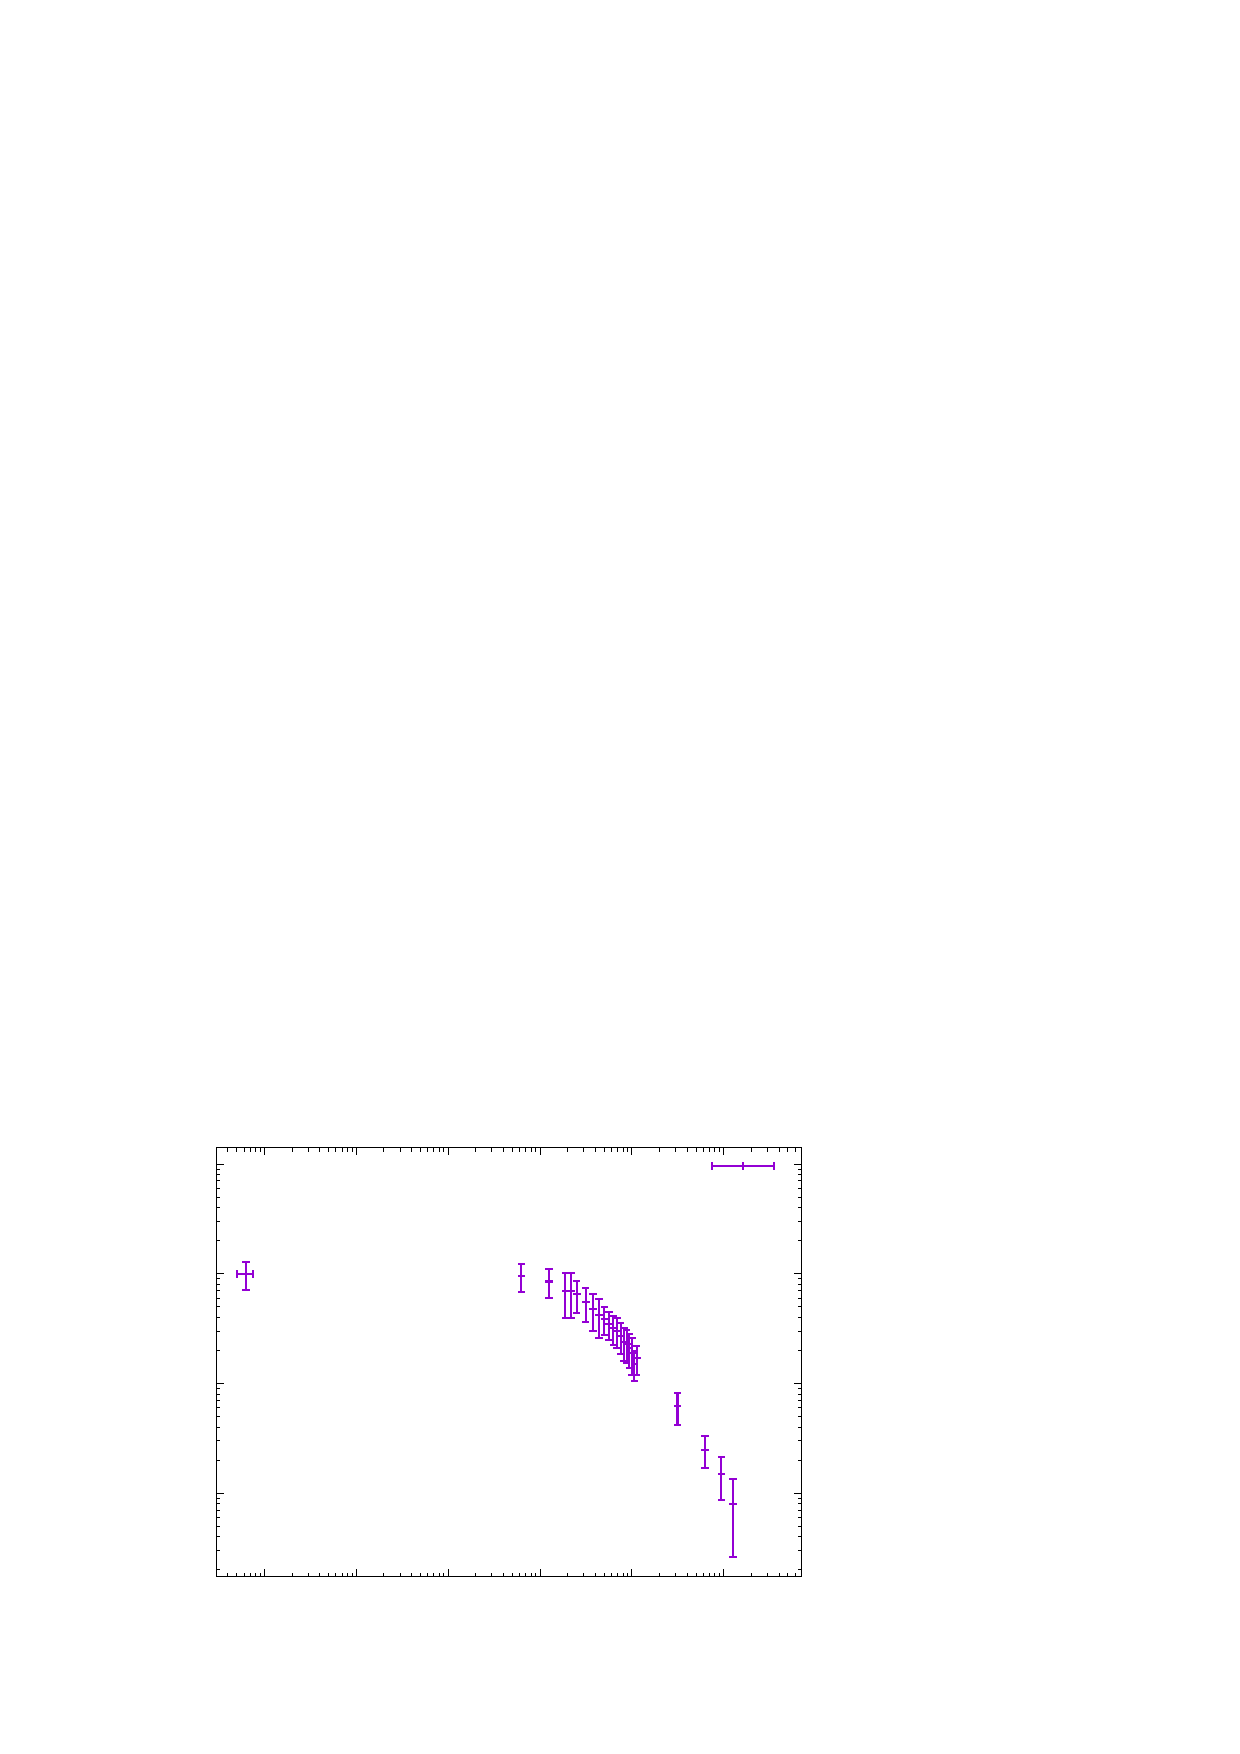
\includegraphics[width={360.00bp},height={252.00bp}]{verstaerkung}}%
    \gplfronttext
  \end{picture}%
\endgroup
}
  \caption{Intensitätsverlauf bei Änderung des Winkels; rot: $\alpha_B$; schwarz: $\alpha_g$}
\end{figure}\newpage
Aus dem Plot ist lassen sich folgende Winkel herauslesen:
\begin{align}
    \alpha_{g1}&=\left(46,25\pm0,2\right)^\circ\\
    \alpha_{g2}&=\left(64,01\pm0,2\right)^\circ\\
    \alpha_{B}&=\left(57,86\pm0,2\right)^\circ\\
\end{align}
$\alpha_{B}$ ist der Brewsterwinkel, hier haben die Minima der Intensität ein Maximum.
Die beiden Grenzwinkel $\alpha_{g1}$ und $\alpha_{g2}$ begrenzen den Bereich, indem die Minima größer werden.
Bei diesen Winkeln gleichen sich die Verluste und die Verstärkung aus.\\

Mithilfe des Brewsterwinkels kann man den Brechungsindex des Glasplättchens berechnen:
\begin{align}
    n&=\tan(\alpha_B)\\
    \Rightarrow\:n&=\left(1,59\pm0,07\right)
\end{align}
Vergleicht man den Wert mit dem Literaturwert des Brechungsindex für Glas, so findet man einen Wert von $1,52$ \citep[vgl.][]{Brechungsindes-Wiki}.
Dieser Wert liegt im Fehlerbereich des berechneten Wertes.
\subsection{Gewinn-Verlust-Bilanz}
Zunächst wird die Gewinn-Verlust-Bilanz der Intensität des Laserstahls beim Durchgang durch folgende Anordnung berechnet werden:
\begin{figure}[h]
    \centering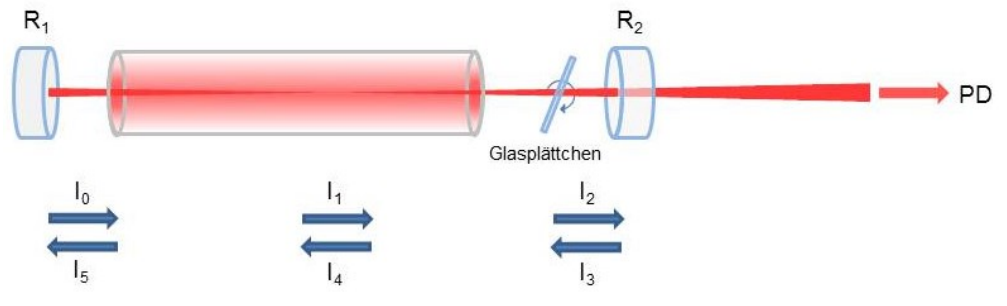
\includegraphics[width=0.7\textwidth]{Auswertung-Dominik/gewinnverlust.PNG}
    \caption{Schematischer Aufbau zur Bestimmung des Verstärkungsfaktor \citep[vgl.][]{Anleitung}}
\end{figure}\\
Dabei sind die Intensitäten wie folgt definiert, wobei $I_6$ parallel zu $I_0$ verläuft.
\begin{align*}
    I_1&=I_0\cdot\exp\left(\nu\cdot l_\text{Medium}\right)\\
    I_2&=I_1\cdot T\\
    I_3&=I_2\cdot R_2\\
    I_4&=I_3\cdot T\\
    I_5&=I_4\cdot\exp\left(\nu\cdot l_\text{Medium}\right)\\
    I_6&=I_5\cdot R_1
\end{align*}
Setzt man nun alle Gleichungen ineinander ein, so erhält man:
\begin{equation}
    I_6=I_0\cdot\left(\exp\left(\nu\cdot l_\text{Medium}\right)\right)^2\cdot T^2\cdot R_1\cdot R_2
\end{equation}
Im Leerlauf ergibt sich $I_6=I_0$, somit folgt für die Verstärkung:
\begin{align}
    I_0&=I_0\cdot\left(\exp\left(\nu\cdot l_\text{Medium}\right)\right)^2\cdot T^2\cdot R_1\cdot R_2\\
    \nu&=\frac{\ln\left(\frac{1}{R_1R_2T^2}\right)}{2\cdot l_\text{Medium}}
\end{align}
Für die Berechnung der Verstärkung sind alle Werte, bis auf den Transmissionskoeffizienten $T$ des Glasplättchens bekannt.
Dieser wird über die Vielstrahl-Interferenz innerhalb des Glasplättchens hergeleitet.
Als Ergebnis, erhält man die sogenannten Airy-Formeln \citep[vgl.][S.86-88]{Laser-Dem}:
\begin{align}
    I_R&=I_0\frac{F\sin^2\left(\delta/2\right)}{1+F\sin^2\left(\delta/2\right)}\\
    I_T&=I_0\frac{1}{1+F\sin^2\left(\delta/2\right)}
\end{align}
Mit der Abkürzung $F=4R/(1-R)^2$.\\
$\delta$ steht hier für die Phasenverschiebung zweier benachbarter Teilstrahlen und lässt sich wie folgt umschreiben:
\begin{equation}
    \delta=2\pi\cdot\frac{\Delta s}{\lambda}+\Delta\Phi = \frac{2\pi}{\lambda}\cdot2d\sqrt{n^2-\sin^2\left(\alpha\right)}+\Delta\Phi
\end{equation}
Der Faktor $\Delta\Phi$ ist der Phasensprung, dieser ist bei einem Etalon aus einem Glasplättchen gleich Null.
Da die Grenzwinkel in einem Minimum bestimm wurden, kann man den Faktor $\sin^2\left(\delta/2\right)$ mit 1 abschätzen.\\
Somit folgt für den Transmissionskoeffizienten:
\begin{align}
    T&=\frac{I_T}{I_0}\\
    T&=\frac{1}{1+F}\\
    T&=\left(\frac{1-R}{1+R}\right)^2
\end{align}
Der Reflexionsgrad kann mithilfe der Fresnel'schen Formeln bestimmt werden:
\begin{align}
    R&=\frac{I_R}{I_0}=\left(\frac{E_R}{E_0}\right)^2\\
    R&=\frac{\tan^2\left(\alpha-\beta\right)}{\tan^2\left(\alpha+\beta\right)}
    %s_R&=\sqrt{\left(s_\alpha\cdot\right)^2+\left(s_\beta\cdot\right)^2}
\end{align}
Der Winkel $\alpha$ ist durch die Messung bekannt, der Winkel $\beta$ kann durch das Snelliussches Brechungsgesetz berechnet werden:
\begin{align}
    \sin(\alpha)&=n\sin\left(\beta\right)\\
    \beta&=\arcsin\left(\frac{\sin\left(\alpha\right)}{n}\right)%\\
   % s_\beta&=\sqrt{\left(s_\alpha\cdot\frac{\cos(\alpha)}{n\cdot\sqrt{1-\frac{\sin^2\left(\alpha\right)}{n^2}}}\right)^2+\left(s_n\cdot\frac{\sin(\alpha)}{n^2\sqrt{1-\frac{sin^2(\alpha)}{n^2}}}\right)^2}
\end{align}
Die Transmission und der Verstärkungsfaktor wird nun an den beiden Grenzwinkeln $\alpha_{g1}$ und $\alpha_{g2}$ berechnet.
Für die Reflexionsgrade der beiden Spiegel wird, wie in der Anleitung, $R_1 = 0,99$ und $R_2 = 0,98$ verwendet und für $l_{Medium} = 0,545$.
\begin{table}[h]
    \centering\begin{tabular}{c|ccccc}
        &$\alpha$/(Grad)&$\beta$/(Grad)& R $\cdot 10^{-3}$ &$T$&$\nu$/(m$^{-1}$)\\\hline
        Grenzwinkel 1&$\left(46,25\pm0,2\right)$&$\left(27,02\pm0,2\right)$&$\left(10,99\pm0,26\right)$&$\left(0,957\pm0,001\right)$&$\left(0,100\pm0,002\right)$\\
        Grenzwinkel 2&$\left(64,01\pm0,2\right)$&$\left(34,43\pm0,3\right)$&$\left(7,09\pm0,47\right)$&$\left(0,972\pm0,002\right)$&$\left(0,072\pm0,003\right)$\\
    \end{tabular}
\end{table}\\
Die Fehler wurden über das Fehlerfortpflanzungsgesetz bestimmt.
Somit erhält man eine durchschnittliche Verstärkung von:
\begin{equation}
    \nu=\left(0,086\pm0,003\right)\,\text{m}^{-1}
\end{equation}\newpage
Um nun herauszufinden, wie genau man die Dicke des Plättchens messen müsste, um (ohne Winkelmessung) die gleiche Genauigkeit zu erhalten, setzt man den Fehler der Winkelmessung mit dem Fehler der Dickenmessung gleich:
\begin{align}
    \frac{\partial \delta}{\partial \alpha}s_\alpha &=\frac{\partial \delta}{\partial d}s_d\\
    \Leftrightarrow s_d&=\frac{d\cos(\alpha)\sin(\alpha)}{n^2-\sin^2(\alpha)}=0,7\,\mu m
\end{align}
Diese Genauigkeit ist mit einer Mikrometerschraube kaum erreichbar (kleinste Skaleneinheit: $5\,\mu m$).
Somit ist die Winkelmethode deutlich genauer.
\subsection{Dicke des Glasplättchens}
Über den Abstand der Maxima können wir auch die Dicke des Glasplättchens bestimmen.
Dies wird mithilfe der Bedingung für konstruktive Interferenz gemacht.
Somit folgt für die Dicke $d$:
\begin{equation}
    d=\left|\frac{\left(k_2-k_1\right)\cdot\lambda}{2\left(\sqrt{n^2-\sin\left(\alpha_{k_1}\right)^2}-\sqrt{n^2-\sin\left(\alpha_{k_2}\right)^2}\right)}\right|
\end{equation}
Hierbei stehen $k_2$ und $k_1$ für die Indizes der entsprechenden Maxima.
Es werden jeweils die benachbarten Maxima, mit einen Winkel kleiner $\alpha_{g1}$ verwendet.
Anschließend wird über alle Werte gemittelt. 
Die einzeln gemessenen Werte finden sich im Anhang.\\
Somit erhalten wir eine Dicke von:
\begin{equation}
    \bar{d}=\left(144,7\pm6,7\right)\,\mu m
\end{equation}
Dies kommt an den in der Versuchsanleitung angegebenen Wert von $150\,\mu m$ heran und ist um einiges genauer, als die Bestimmung über die Schwebungsfrequenz bei den axialen Moden.
\newpage